\chapter{Methodology} \label{sec:methodology}

Here describe the methodology you use and why you decided to use it.
e.g., theoretical considerations, simualtons, experiments, measurements, testbeds, emulations, etc. What concepts are used.

Also explain which metrics you use to measure success or failure (e.g., detection performance with accuracy, recall, precision, f1 score, RocAUC, etc.)


Provide a figure (see example figure \ref{fig:modeling-example}) to describe the processing steps

\begin{figure}[h]
	\centering
	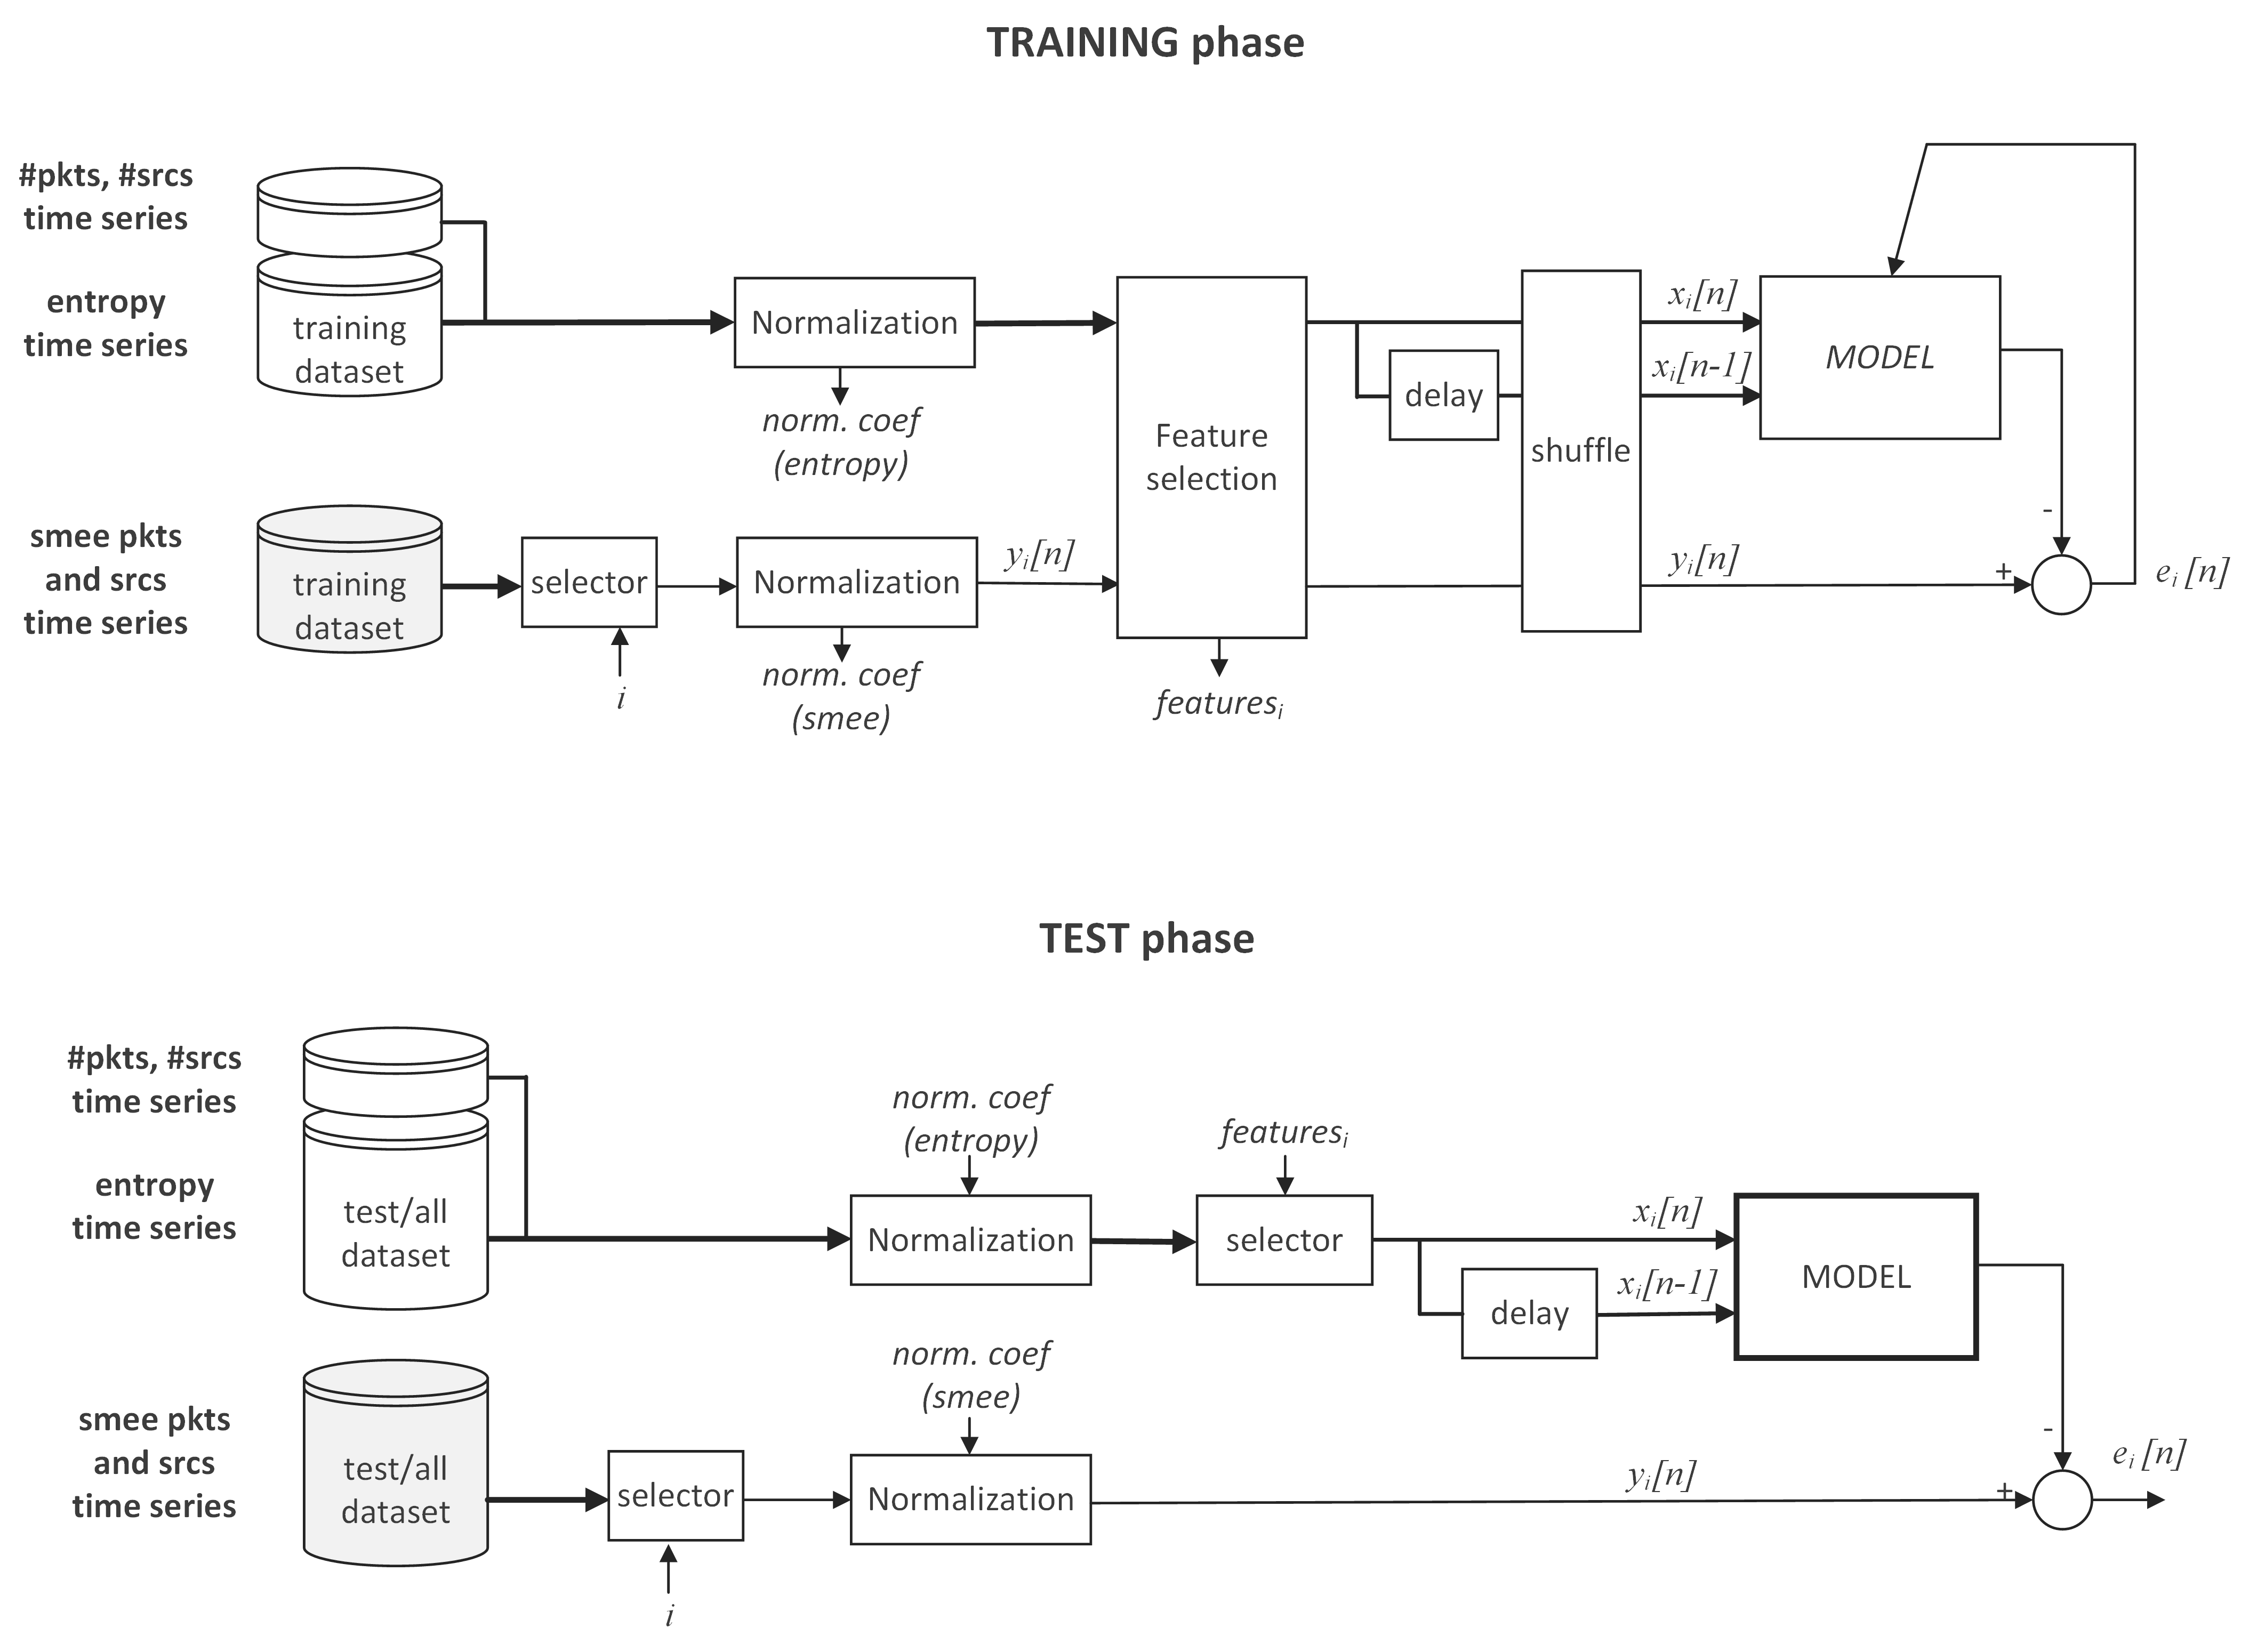
\includegraphics[width=0.95\linewidth]{graphics/modeling-example}
	\caption{Describe in the caption exactly what can be seen in the figure}
	\label{fig:modeling-example}
\end{figure}




\newpage